\documentclass[conference]{IEEEtran}
\IEEEoverridecommandlockouts
% Template version as of 6/28/2024 (blockarch2026Template)

\usepackage{cite}
\usepackage{amsmath,amssymb,amsfonts}
\usepackage{algorithmic}
\usepackage{algorithm}
\usepackage{array}
\usepackage[caption=false,font=normalsize,labelfont=sf,textfont=sf]{subfig}
\usepackage{textcomp}
\usepackage{url}
\usepackage{verbatim}
\usepackage{graphicx}
\usepackage{xcolor}
\usepackage{hyperref}
\hyphenation{op-tical net-works semi-conduc-tor IEEE-Xplore}
\def\BibTeX{{\rm B\kern-.05em{\sc i\kern-.025em b}\kern-.08em
    T\kern-.1667em\lower.7ex\hbox{E}\kern-.125emX}}

% ============================================
% DOCUMENT BEGINS
% ============================================
\begin{document}

\title{A Lock Free, Non-blocking, In Line Processing Architecture for High Throughput and Regulatory Compliant Blockchain Trading Applications}

\author{
\IEEEauthorblockN{Dr. Andrew Le Gear}
\IEEEauthorblockA{CSIS Department,\\Bernal Institute,\\University of Limerick, Ireland\\andrew.p.legear@ul.ie}
\and
\IEEEauthorblockN{Prof. Jim Buckley}
\IEEEauthorblockA{CSIS Department,\\Lero,\\University of Limerick, Ireland\\jim.buckley@ul.ie}
\and
\IEEEauthorblockN{Tawny Whatmore}
\IEEEauthorblockA{Horizon Globex Ireland,\\Ireland\\tawny.whatmore@horizon-globex.ie}
\and
\IEEEauthorblockN{Dr. Ashish Sai}
\IEEEauthorblockA{Department of Advanced Computing Sciences\\Maastricht University, Netherlands\\ashish.sai@maastrichtuniversity.nl}
}

% The paper headers
\markboth{IEEE ICBC 2026, Brisbane, Australia, 1--5 June 2026}%
{Le Gear \MakeLowercase{\textit{et al.}}: Lock Free Blockchain Trading Architecture}

\maketitle

% ============================================
% INCLUDE SECTIONS
% ============================================

% ============================================
% ABSTRACT
% ============================================
\begin{abstract}
Regulated DeFi demands blockchain trading systems that satisfy both high-throughput performance and regulatory compliance. We present an empirical analysis of architectural patterns for high-throughput blockchain trading, based on a production system deployed for live trading operations. Using a two-layer hybrid model separating off-chain compliance from on-chain settlement, we conduct an ablation study of five architectural variants. Our symbol-sharded, lock-free architecture achieves 31.19 tx/sec—a \textbf{2.8$\times$ improvement} over conventional designs and 125-fold gain from naive baselines.

Our analysis reveals migrating bottlenecks: resolving blockchain constraints exposes server-side crises. Ethereum's nonce mechanism limits naive parallelism to 36\% throughput gain, while circumventing it with multiple wallets causes 9$\times$ latency increases due to lock contention. Our lock-free transaction submission model, inspired by HFT architectures, reduces latency by 44\% while maintaining peak throughput, demonstrating that holistic co-design of on-chain and off-chain components is essential for optimal performance.
\end{abstract}

% ============================================
% KEYWORDS
% ============================================
\begin{IEEEkeywords}
Blockchain, Regulated DeFi, lock-free concurrency, high-frequency trading, regulatory compliance, transaction throughput, symbol sharding.
\end{IEEEkeywords}

% ============================================
% I. INTRODUCTION
% ============================================
\section{Introduction}
\label{sec:intro}

Decentralized finance (DeFi) and traditional financial markets have converged to create Regulated DeFi (R-DeFi), which seeks to harness blockchain's transparency and immutability while adhering to regulatory frameworks~\cite{zetzsche2020defi,jamithireddy2025hybrid}. A core tension underpins this space: compliance requirements (Know Your Customer/KYC, Anti-Money Laundering/AML, trade surveillance) are computationally intensive and require confidential off-chain data, making them ill-suited for direct on-chain implementation~\cite{sak2024kyc,wolfsberg2022framework}.

Public blockchains like Ethereum process only 15--30~tx/sec on their base layer~\cite{schaffer2019performance,xu2021slimchain}, and embedding stateful compliance logic on-chain is prohibitively slow and expensive~\cite{eren2025onchain}. This creates an ``all or nothing'' dilemma: full decentralization with non-compliance, or centralization that sacrifices blockchain's auditability. Hybrid architectures offer a pragmatic middle ground~\cite{zhu2026hybrid}.

We advocate a two-layer hybrid architecture that separates responsibilities between an off-chain server and an on-chain ledger. The off-chain layer serves as a high-performance compliance and order matching engine, while the blockchain handles immutable, final settlement. This mirrors established enterprise adoption patterns where the blockchain acts as a shared, trusted backend rather than a world computer~\cite{jamithireddy2025hybrid}. Importantly, this is not merely theoretical: our industrial partner, Horizon Globex Ireland, deploys \textbf{Architecture~5} (the symbol-sharded, lock-free design) in production for the Horizon Globex trading platform. Our empirical study uses a dedicated test environment replicating this production system, allowing rigorous performance analysis without affecting live operations. Yet even this separation introduces non-trivial performance bottlenecks in the transaction submission pipeline, an area we address through the following research questions:

\begin{itemize}
    \item \textbf{RQ1:} What throughput ceiling does a two-layer hybrid blockchain trading architecture face given gas-based block limits and regulatory constraints, and what are the primary bottlenecks that shift as the system is optimized?
    \item \textbf{RQ2:} How can lock-free concurrency patterns from high-frequency trading (HFT) be adapted to the unique constraints of blockchain transaction submission, such as nonce sequencing?
    \item \textbf{RQ3:} What is the relationship between architectural design choices in the submission layer and the end-to-end latency of trade settlement?
\end{itemize}

We present a systematic ablation study of five distinct architectural variants, from a naive synchronous baseline to a highly optimized, lock-free, symbol-sharded design. Our contributions include:

\begin{enumerate}
    \item A two-layer hybrid architecture for R-DeFi featuring a symbol-sharded, lock-free transaction submission model that balances regulatory compliance, high-throughput performance, and decentralization principles, currently deployed in live trading environments.
    \item Empirical evidence that this architecture achieves 31.19~tx/sec, a \textbf{2.8$\times$ improvement} over conventional asynchronous multi-threaded architectures, with the submission layer sustaining rates exceeding the blockchain's gas-based theoretical capacity.
    \item A systematic ablation study isolating and quantifying performance bottlenecks, revealing how resolving one constraint can expose another. Most notably, we observe a 9$\times$ latency increase when a blockchain bottleneck was removed.
    \item Evidence that on-chain nonce contention limits naive parallelism to a 36\% throughput gain, validating Amdahl's Law in a blockchain context~\cite{amdahl1967validity}.
    \item The first documented empirical evidence of server-side contention emerging directly from successful resolution of a blockchain-side bottleneck, a finding with implications for future system designers.
\end{enumerate}



% ============================================
% II. RELATED WORK AND BACKGROUND
% ============================================
\section{Related Work and Background}
\label{sec:related}

This work draws on three domains: blockchain scalability, concurrent system design, and high-frequency trading. We review prior work informing our experimental findings.

\subsection{Blockchain Scalability and Sharding}

Public blockchains face well-documented performance limitations~\cite{bez2019scalability,ucbas2023performance}. These studies attribute Ethereum's low throughput to inherent trade-offs between decentralization, security, and scalability, providing a theoretical model for the bottlenecks our baseline architecture empirically demonstrates at 0.25~tx/sec. Sharding, a technique for partitioning state across nodes, is a primary approach to address these limitations~\cite{fynn2018partitioning}. Our symbol-sharded architecture leverages domain-specific partitioning that avoids cross-shard communication overhead; empirical results are presented in Section~\ref{sec:results}.

\subsection{Nonce Contention and Parallelization Limits}

Nonce contention poses a key bottleneck in Ethereum transaction submission. The nonce mechanism requires strict sequential ordering per account, limiting parallelization~\cite{hu2023nonce}. As shown in Section~\ref{sec:results}, multi-threading against a single wallet yields only a modest throughput gain, empirically confirming this limitation. Alternative concurrency models, such as Paimani's ``wait-free'' approach~\cite{paimani2021sonicchain}, address contention through delegation, but our multi-wallet partitioning offers a more direct strategy, though it shifts the bottleneck to server-side contention if not managed with appropriate lock-free controls.

\subsection{Lock-Free Architectures from High-Frequency Trading}

Our approach to resolving server-side contention draws from high-frequency trading (HFT) principles. Cache thrashing and lock convoying are phenomena HFT systems carefully avoid~\cite{moir2018concurrent}. We apply the \textbf{LMAX Disruptor pattern}~\cite{thompson2011disruptor}, a lock-free ring buffer achieving sub-microsecond latency in traditional finance. As demonstrated in Section~\ref{sec:results}, adapting these techniques via symbol-sharded, lock-free queues overcomes blockchain-specific performance barriers~\cite{bilokon2023cpp,ng2018lockfree}.

\subsection{Research Gap}

Platform-level blockchain scalability research is extensive, but systematic application level analysis isolating specific bottlenecks (nonce contention, server-side locking) remains sparse. Lock-free HFT architectures have not been widely adapted to blockchain's unique constraints, and how submission-layer design affects end-to-end settlement latency lacks empirical characterization. Our ablation study addresses these gaps.


% ============================================
% III. SYSTEM ARCHITECTURE AND REGULATORY CONSTRAINTS
% ============================================
\section{System Architecture and Regulatory Constraints}
\label{sec:architecture}

Horizon Globex Ireland DAC is a fintech software services company operating blockchain-backed trading and exchange systems across multiple jurisdictions. Its deployments include automated trading systems in the United States and the Upstream platform in the Seychelles, which supports MERJ, a tier-one regulated stock exchange. Its core offering is a suite of blockchain-backed market trading and securities software services designed to satisfy the compliance requirements of regulated financial markets. The architecture described in this paper was designed to meet the throughput and regulatory demands of this production environment.

Our proposed system employs a two-layer hybrid architecture designed to balance high-performance trading demands with stringent regulatory requirements. This model segregates responsibilities between a high-throughput off-chain server and a secure on-chain settlement layer, consistent with emerging patterns in enterprise blockchain adoption~\cite{jamithireddy2025hybrid}. This architecture represents our \textbf{first contribution (C1)} and directly addresses \textbf{RQ1}: characterizing the throughput ceiling imposed by gas-based block limits under compliance requirements.

\subsection{Two-Layer Architectural Model}

\textbf{Layer 1: Off-Chain Order Management Server.} This layer is a centralized, high-performance server responsible for all real-time trading operations. Its duties include user authentication, order ingestion, compliance checks (e.g., KYC/AML, trading limits), order matching, and maintaining the live order book. By handling these operations off-chain, we leverage the speed and scalability of traditional centralized systems for tasks that do not require immediate blockchain consensus, a common strategy in Layer 2 scaling solutions~\cite{xu2021slimchain}.

\textbf{Layer 2: On-Chain Settlement and Finality Layer.} This layer consists of a private, permissioned Ethereum-based blockchain network running an IBFT 2.0 consensus mechanism. Its sole responsibility is to provide a secure, immutable, and auditable ledger for the final settlement of matched trades. The \texttt{ATS.sol} smart contract serves as the on-chain automated trading system, providing a simple \texttt{bid} function to record the settlement of a trade.

\subsection{Data Flow and Justification}

The data flow proceeds as follows: (1)~clients submit orders to the off-chain server; (2)~the server validates against compliance rules and matches against the order book; (3)~matched trades are submitted to the \texttt{ATS.sol} smart contract; (4)~IBFT~2.0 consensus provides finality and a tamper-proof audit trail~\cite{kuhn2019rethinking}. The two-layer model is illustrated in Figure~\ref{fig:architecture}(a).

Table~\ref{tab:architecture-justification} summarizes the key benefits of this hybrid design.

\begin{table}[htbp]
\centering
\caption{Justification for the Hybrid Architecture}
\label{tab:architecture-justification}
\begin{tabular}{@{}p{0.18\textwidth}p{0.75\textwidth}@{}}
\toprule
\textbf{Factor} & \textbf{Benefit} \\
\midrule
Regulatory Compliance & Enforces KYC/AML checks \textit{before} immutable recording~\cite{fincen2024kyc}; enables pre-trade enforcement vs.\ post-facto in decentralized models \\
\addlinespace
Performance & Reserves blockchain throughput for settlement; Architecture~1 baseline (0.25~tx/sec) confirms on-chain-only is unworkable~\cite{khan2021blockchain} \\
\addlinespace
Cost-Effectiveness & Minimizes on-chain transactions, reducing computational load and enabling higher settlement throughput \\
\addlinespace
Data Privacy & Protects open order privacy; only settled trades are broadcast to the blockchain \\
\bottomrule
\end{tabular}
\end{table}

% ============================================
% IV. THE NOVEL HIGH-THROUGHPUT COMPONENTS
% ============================================
\section{The Novel High-Throughput Components}
\label{sec:components}

We introduce two components for high-throughput parallel processing: the \textbf{Asynchronous Multi-Wallet Strategy} and the \textbf{Symbol-Sharded Lock-Free Model}. Together, these address blockchain-level nonce bottlenecks and server-side contention by adapting HFT lock-free concurrency patterns to blockchain's nonce constraints.

\subsection{Asynchronous Multi-Wallet Strategy}

Ethereum's sequential nonce requirement forces all transactions from a single wallet into strict serial order~\cite{wood2014yellowpaper}. Our strategy creates a one-to-one mapping between trading symbols and dedicated wallets, enabling independent transaction lanes. Trades for different symbols use separate nonce sequences, breaking the single-wallet bottleneck, as the results in Section~\ref{sec:results} demonstrate.

\subsection{Symbol-Sharded Lock-Free Model}

Multi-wallet solves the on-chain bottleneck, but Architecture~4 showed it shifts contention to the server (latency increased from 2.9s to 27.2s). The Symbol-Sharded Lock-Free Model extends symbol-based parallelism to internal data structures using dedicated, lock-free concurrent queues per symbol:

\begin{enumerate}
    \item \textbf{Routing:} Incoming trades route immediately to symbol-specific queues.
    \item \textbf{Parallel Consumption:} Dedicated worker threads consume from each symbol's queue.
    \item \textbf{Lock-Free Processing:} .NET's \texttt{ConcurrentQueue<T>} (Michael-Scott algorithm~\cite{michael1996lockfree}) uses CAS operations instead of locks, ensuring non-blocking, thread-safe operations.
    \item \textbf{Dedicated Submission:} Each worker uses its symbol's dedicated wallet for blockchain submission.
\end{enumerate}

This end-to-end symbol-sharded architecture eliminates server-side contention, reducing latency by 44\% (27.2s$\rightarrow$15.4s). Combined, these components achieve 31.19~tx/sec (\textbf{2.8$\times$} over conventional designs), ensuring the submission layer sustains rates exceeding blockchain capacity (\textbf{contribution C1}).

\begin{figure}[!ht]
    \centering
    \begin{subfigure}[b]{0.38\textwidth}
        \centering
        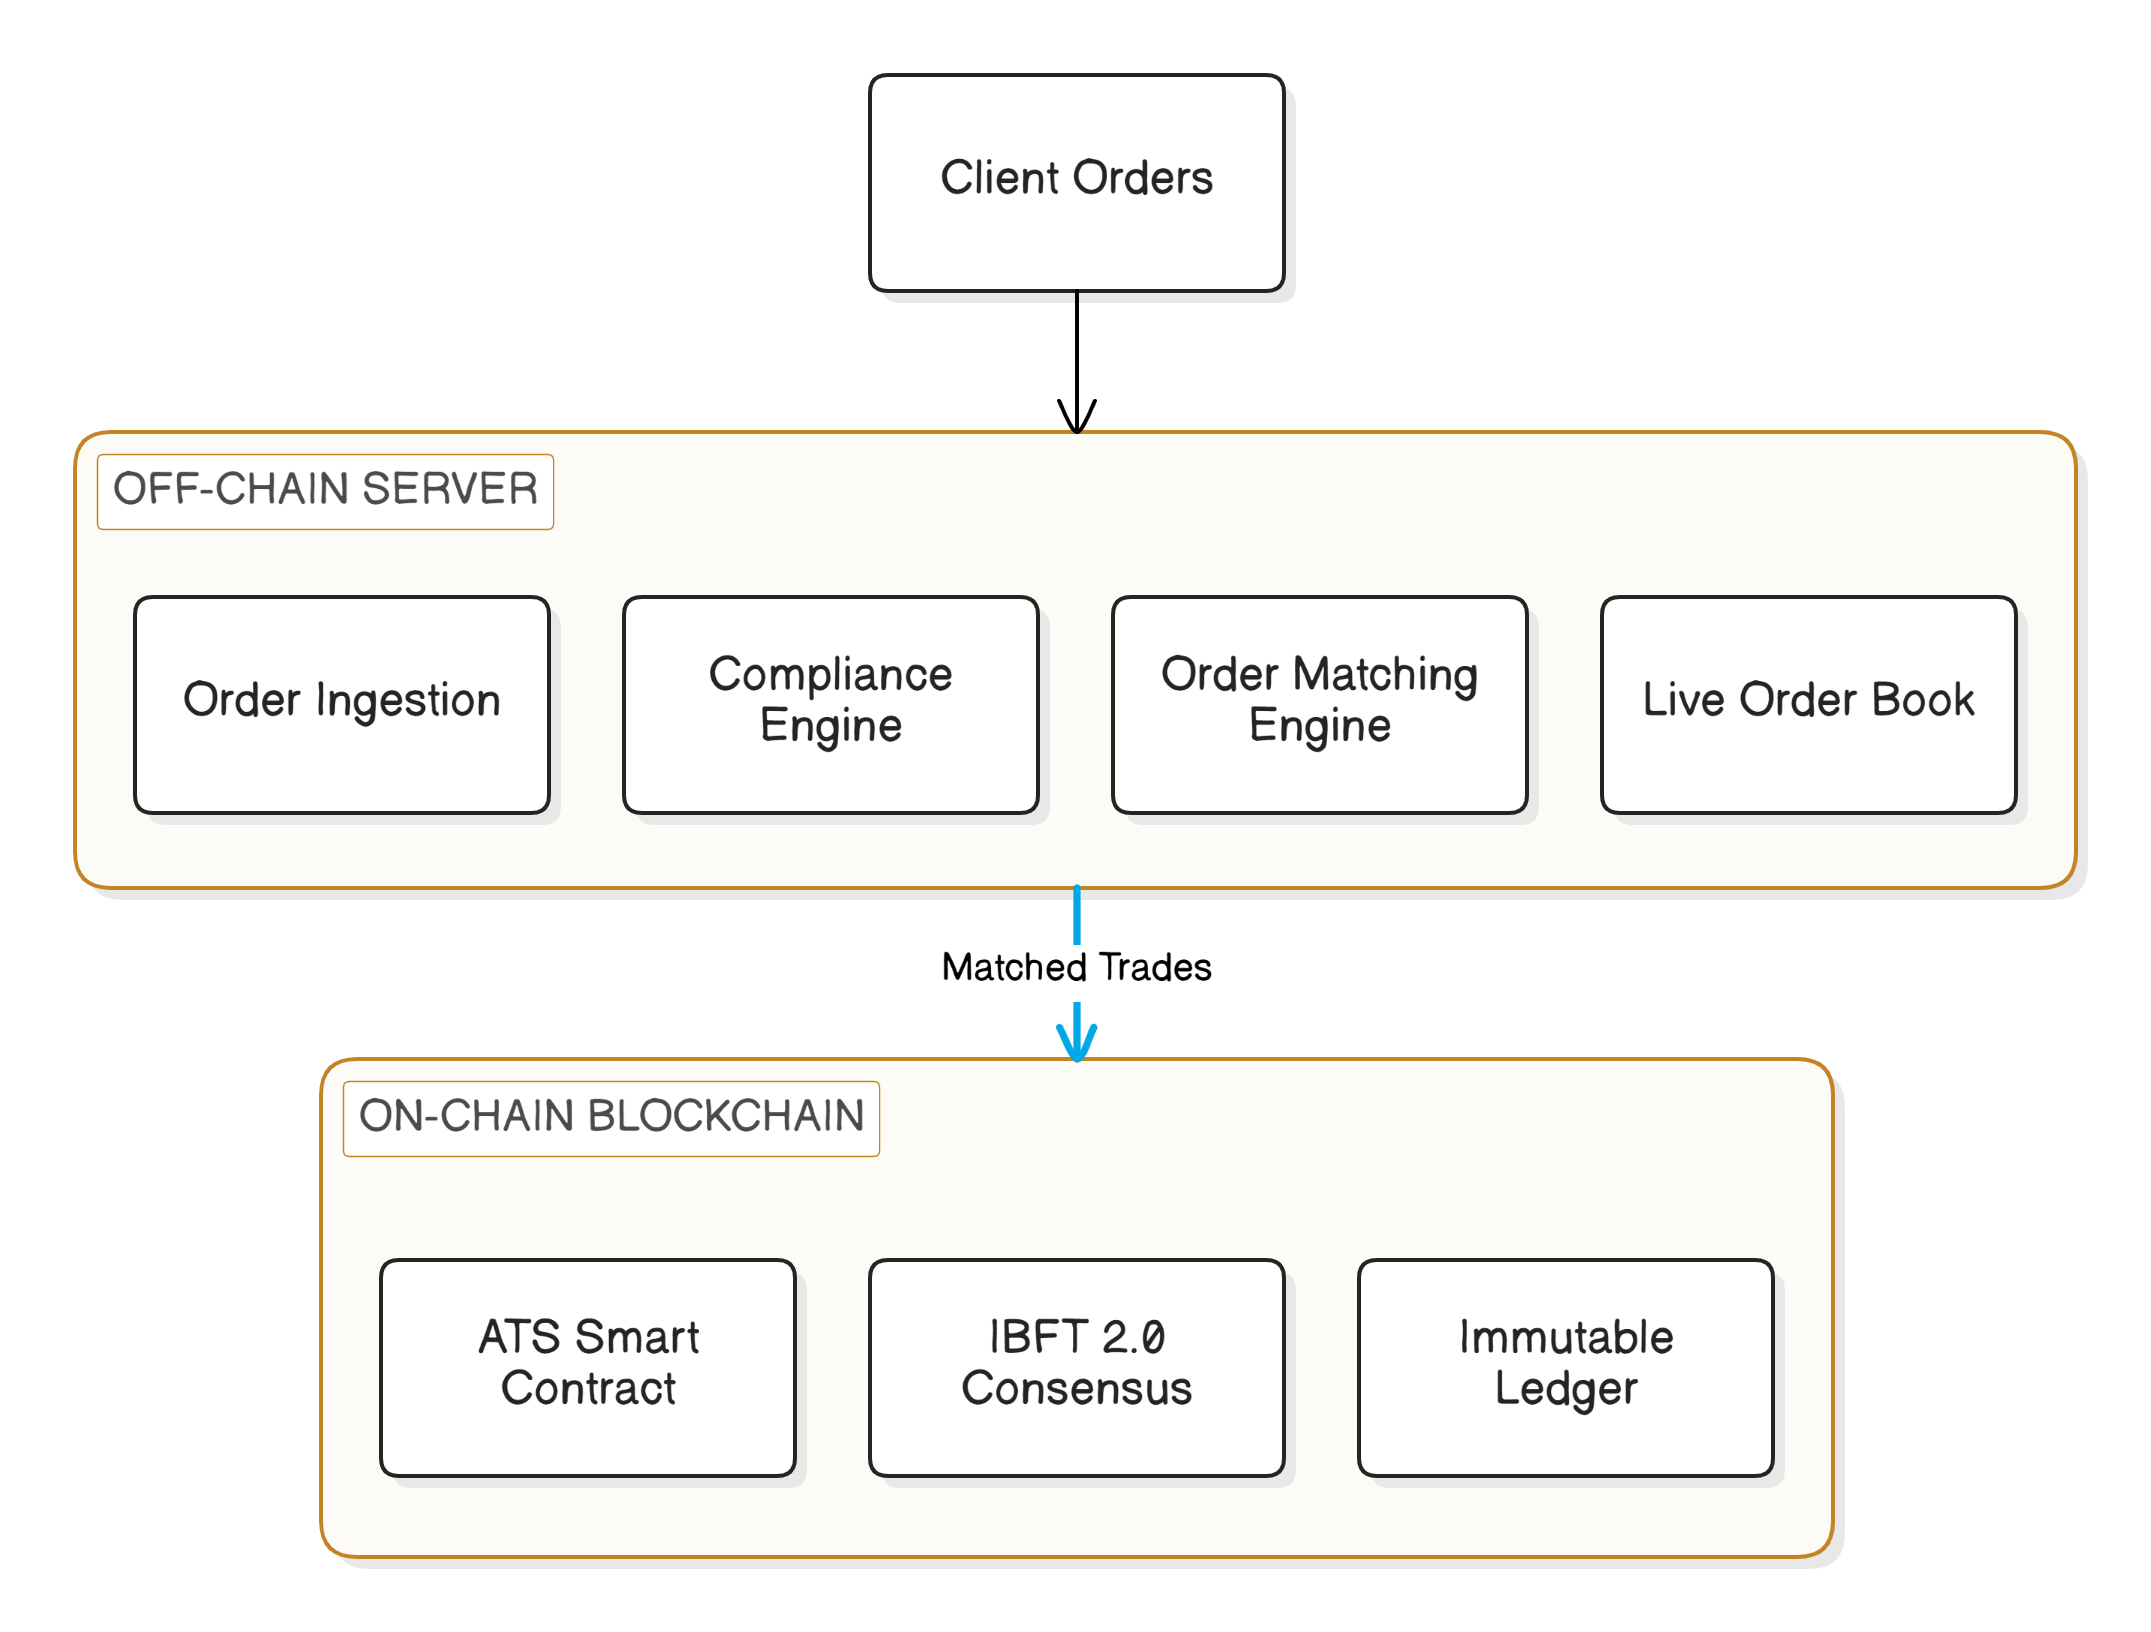
\includegraphics[width=\textwidth]{images/two-layer-model.png}
        \caption{Two-Layer Hybrid Architecture}
        \label{fig:two_layer_model}
    \end{subfigure}
    \hfill
    \begin{subfigure}[b]{0.38\textwidth}
        \centering
        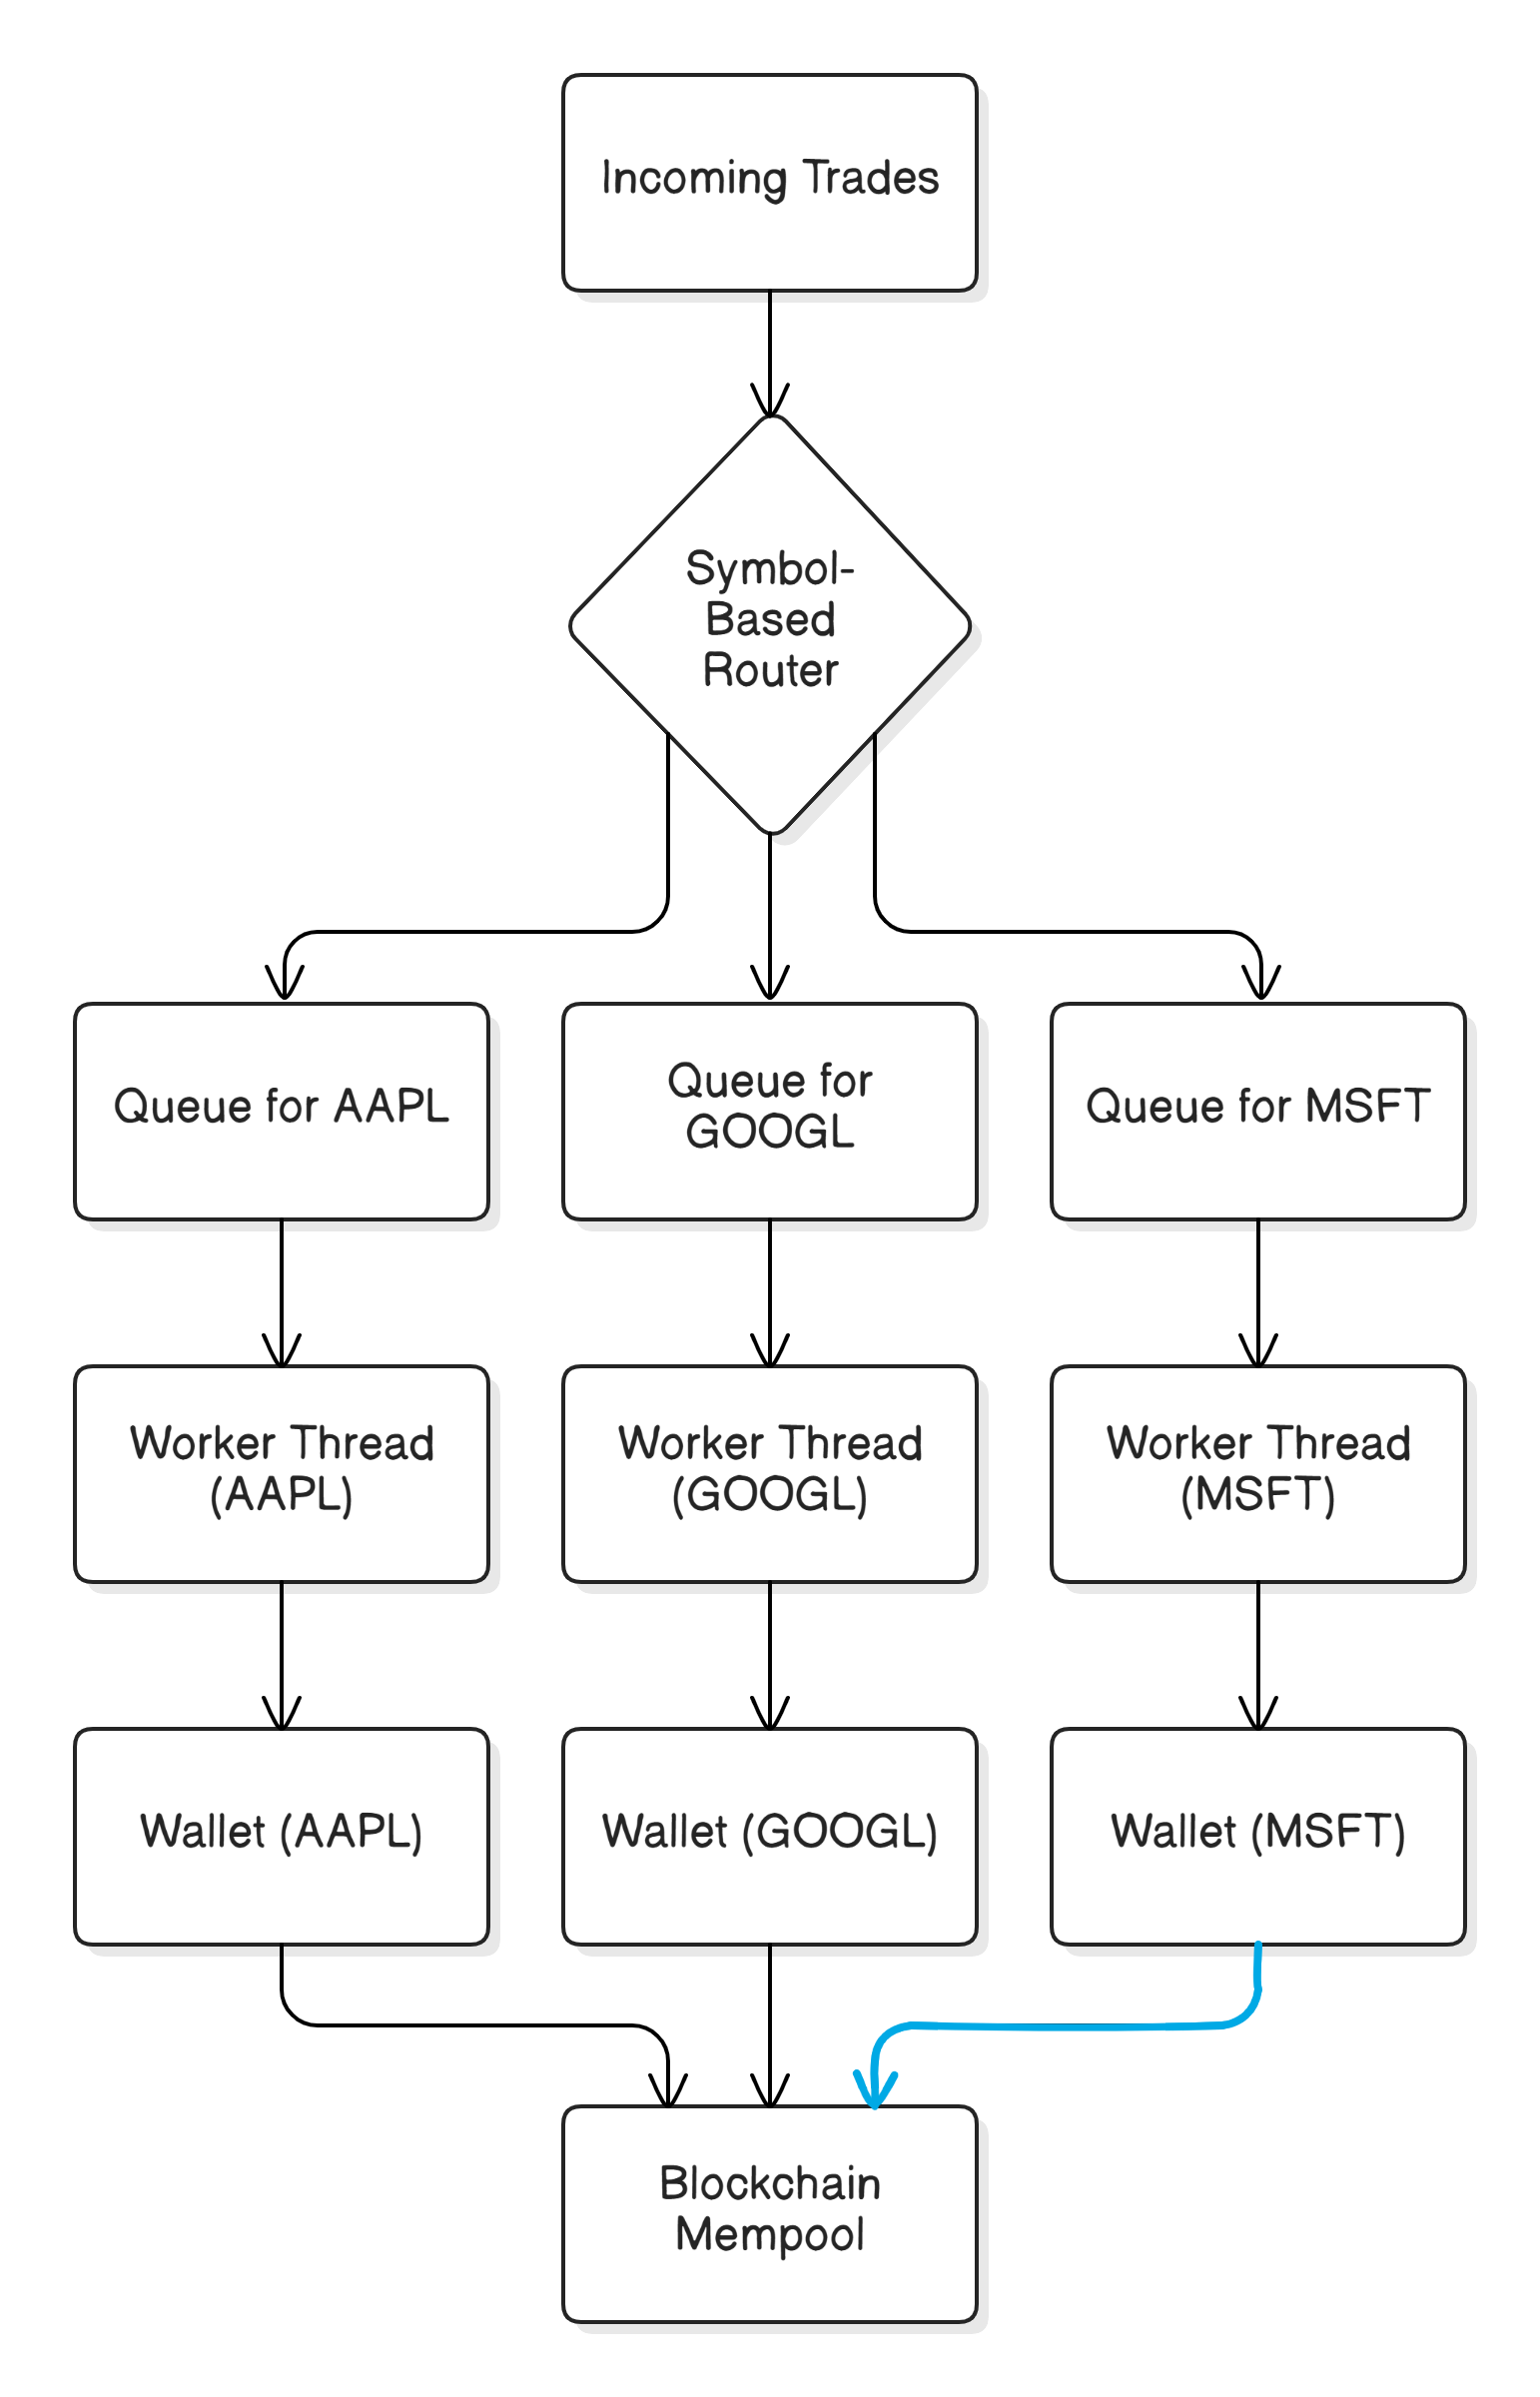
\includegraphics[width=\textwidth]{images/symbol-sharded-lock-free-model.png}
        \caption{Symbol-Sharded Lock-Free Model}
        \label{fig:symbol_sharded_model}
    \end{subfigure}
    \caption{System architecture: (a) Two-layer model separating off-chain compliance from on-chain settlement, (b) Symbol-sharded lock-free model showing end-to-end alignment from symbol queues to dedicated wallets. In both diagrams, rectangles denote processing components and arrows indicate data flow direction; the diamond in~(b) denotes the symbol-based routing decision.}
    \label{fig:architecture}
\end{figure}

% ============================================
% VI. THEORETICAL MAXIMUM THROUGHPUT ANALYSIS
% ============================================
\section{Theoretical Maximum Throughput Analysis}
\label{sec:theoretical}

We formalize a throughput model accounting for both server-side processing and on-chain settlement constraints. The maximum throughput is determined by the minimum of these capacities~\cite{harcholbalter2013performance}:

\begin{equation}
\lambda_{max} = \min(\lambda_{server}, \lambda_{blockchain})
\label{eq:lambda_max}
\end{equation}

\textbf{Blockchain-Side Limit.} The blockchain throughput is constrained by block gas limit ($G_{block}$), gas cost per transaction ($G_{tx}$), and block time ($T_{block}$). With our configuration (10,485,760 gas limit, 4-second blocks, 146,194 gas/tx):

\noindent
\begin{minipage}{0.48\textwidth}
\begin{equation}
\lambda_{blockchain} = \frac{G_{block}}{G_{tx} \cdot T_{block}}
\end{equation}
\end{minipage}%
\hfill
\begin{minipage}{0.48\textwidth}
\begin{equation}
\lambda_{blockchain} = \frac{10{,}485{,}760}{146{,}194 \times 4} \approx 17.93 \text{ tx/sec}
\end{equation}
\end{minipage}

This represents the \textit{sustained} throughput ceiling—the maximum rate at which transactions can be confirmed indefinitely in steady state. However, our observed throughput in Architecture~5 was 31.19~tx/sec with 125 transactions per block, significantly exceeding this limit. This demonstrates the architecture's \textbf{burst handling capability}.

The distinction between \textit{sustained} and \textit{burst} throughput is critical. Trading workloads are inherently bursty: market events generate sudden spikes far exceeding average rates. When transactions arrive faster than the blockchain's sustained capacity, they accumulate in the mempool and confirm across subsequent blocks. Our measured 31.19~tx/sec reflects transactions \textit{submitted and eventually confirmed} over the test duration—1.74$\times$ the sustained capacity (31.19/17.93). In sustained load exceeding 17.93~tx/sec, throughput would converge toward this ceiling as the mempool reaches equilibrium. The key insight: our architecture shifted the bottleneck away from server-side contention, processing transactions faster than the blockchain could confirm them.

\textbf{Server-Side Limit.} Server throughput depends on parallelism and synchronization costs, following Amdahl's Law~\cite{gustafson1988reevaluating} and Little's Law~\cite{little1961proof}:

\begin{equation}
\lambda_{server} = \frac{N}{T_{process} + T_{contention}}
\end{equation}

where $N$ is parallel workers, $T_{process}$ is per-transaction processing time, and $T_{contention}$ is time waiting for shared resources. Architecture~3 (Multi-Threaded, Single-Wallet) had threads contending for the single wallet's nonce, serializing submissions. Architecture~4 (Unsynchronized Multi-Wallet) removed nonce contention but exposed significant server-side contention, with $T_{contention}$ causing 27.2~s average latency.

\textbf{Achieving Theoretical Maximum.} Our components maximize $\lambda_{server}$ so the system becomes purely blockchain-limited. The \textbf{Asynchronous Multi-Wallet Strategy} creates $N$ independent submission lanes, fully utilizing block gas in parallel. The \textbf{Symbol-Sharded Lock-Free Model} partitions processing by symbol, eliminating inter-thread contention ($T_{contention} \to 0$):

\begin{equation}
\lambda_{server} \approx \sum_{i=1}^{N_{shards}} \frac{1}{T_{process, i}}
\end{equation}

Figure~\ref{fig:solution-architecture} shows the complete integrated architecture combining these components.

\begin{figure}[!ht]
\centering
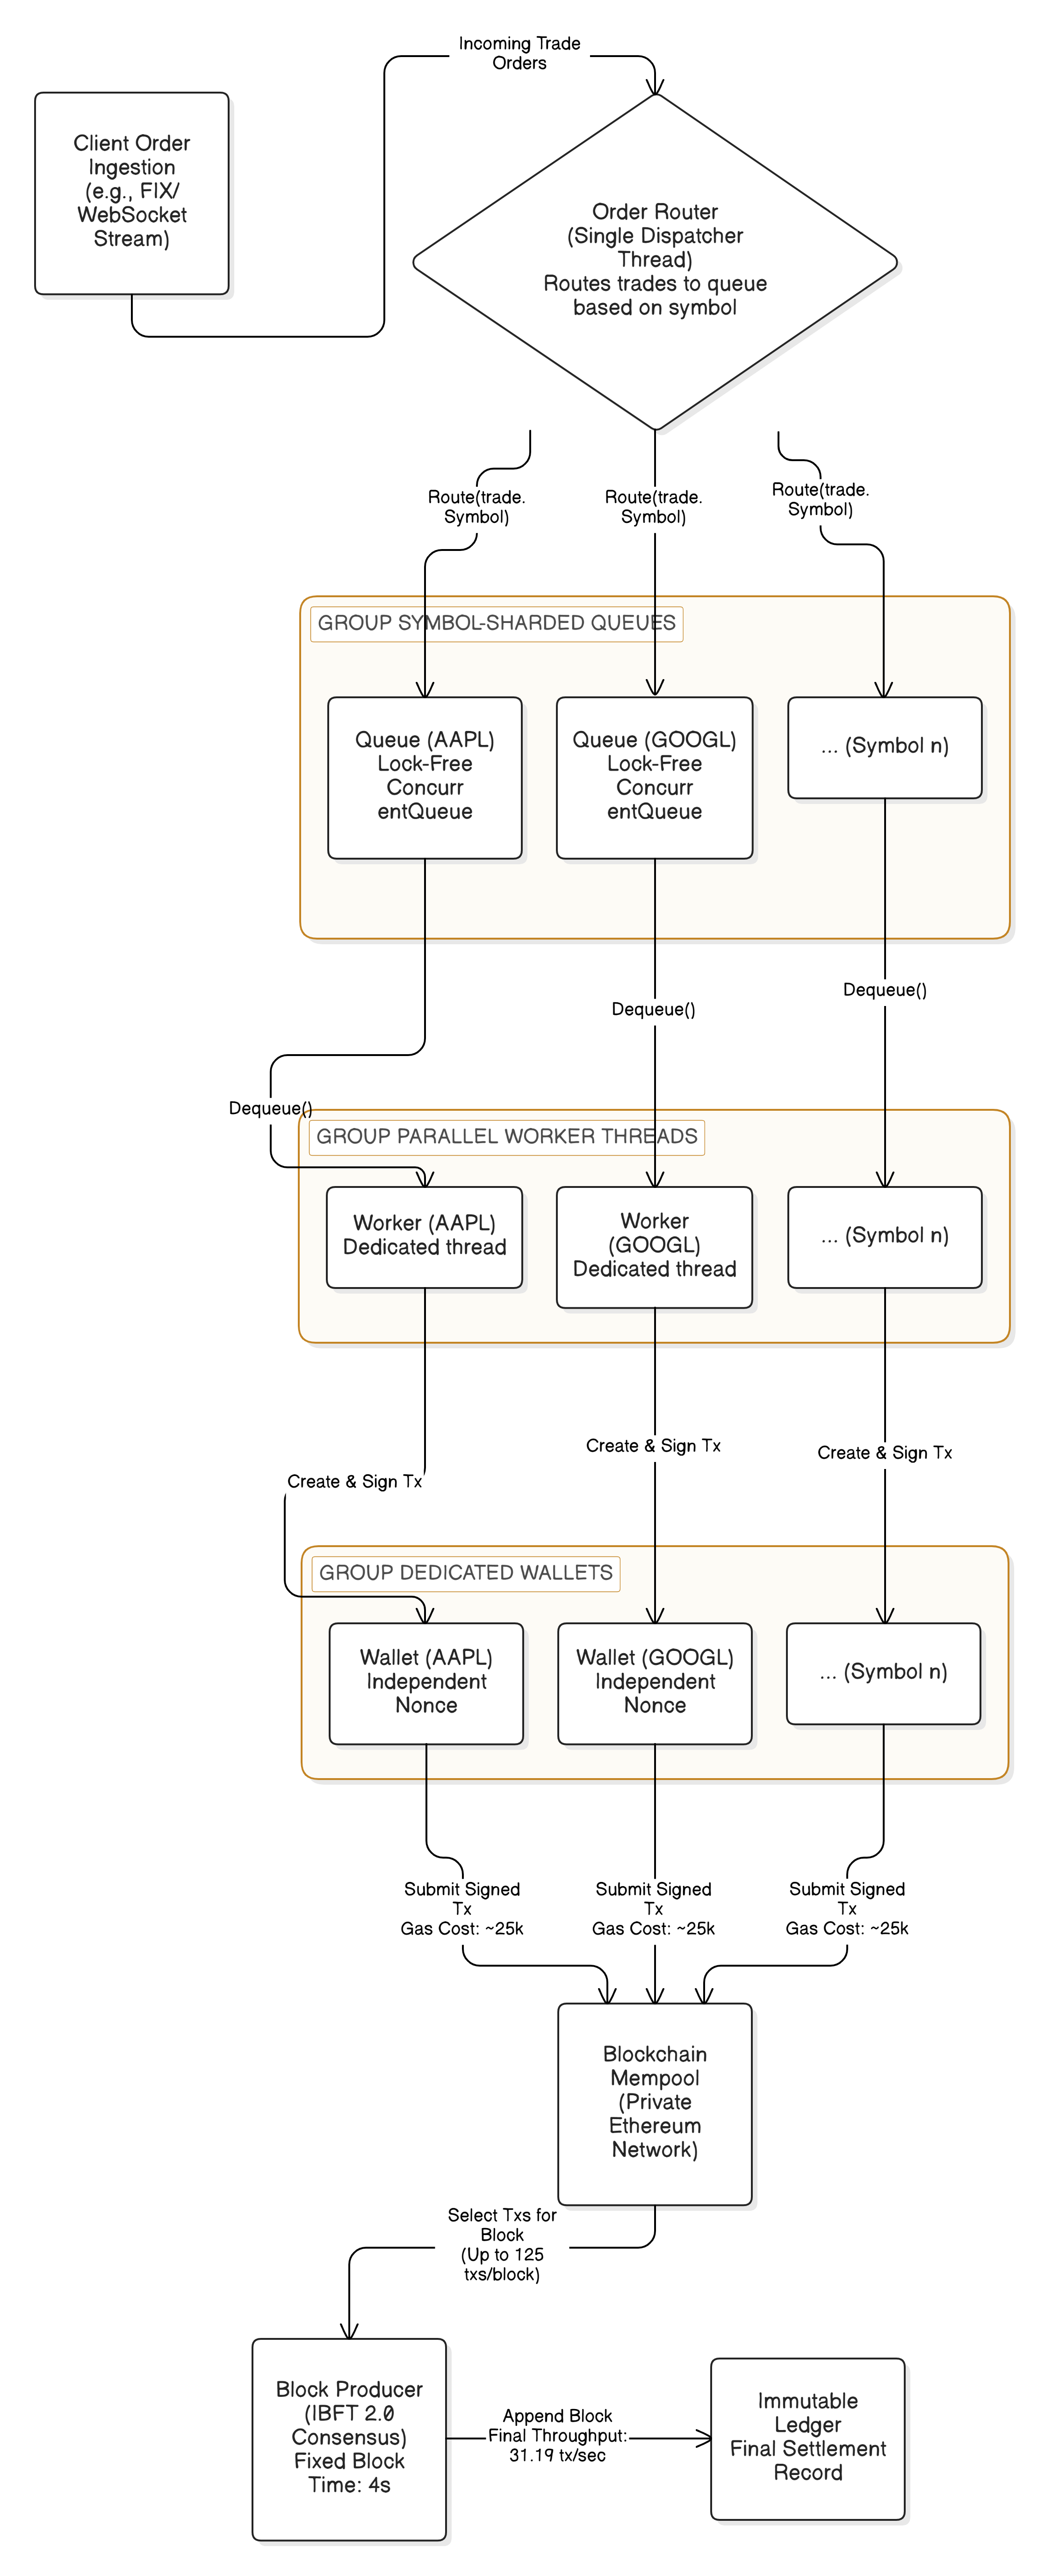
\includegraphics[height=0.65\textheight,keepaspectratio]{images/solution-architecture5.png}
\caption{Complete solution architecture integrating the Symbol-Sharded Lock-Free Model and the Asynchronous Multi-Wallet Strategy, achieving $\lambda_{max} = \lambda_{blockchain}$.}
\label{fig:solution-architecture}
\end{figure}

% ============================================
% V. EXPERIMENTAL METHODOLOGY
% ============================================
\section{Experimental Methodology}
\label{sec:methodology}

We designed an incremental ablation study to evaluate our proposed architecture. Ablation studies, originally developed in neuroscience to understand complex biological systems, have become a standard methodology in systems research for isolating the performance impact of individual components~\cite{meyes2019ablation}. Each stage introduces one key optimization, precisely isolating the impact of distinct bottlenecks: network I/O, nonce contention, and server-side locking. This methodology directly supports \textbf{contribution C3}: a systematic ablation study that isolates and quantifies performance bottlenecks, demonstrating how resolving one constraint can expose another.

The ablation study methodology is particularly well-suited to our research goals. Rather than attempting to optimize all components simultaneously, which would make it difficult to understand which optimizations actually matter, we systematically remove constraints one at a time. This approach, grounded in established performance evaluation practices~\cite{john2007performance}, allows us to identify which component is the limiting factor at each stage, then address it in the next iteration.

\subsection{Architectural Configurations}

We tested five configurations, each introducing one key change from its predecessor:

\textbf{Architecture~1 (Baseline):} Single-threaded, synchronous submission with blocking confirmation. This establishes the performance floor bounded by block time.

\textbf{Architecture~2:} Decouples submission from confirmation via background polling. This isolates the benefit of asynchronous I/O.

\textbf{Architecture~3:} Adds multi-threading to a single wallet. This tests whether parallelism helps despite nonce serialization.

\textbf{Architecture~4:} Introduces a multi-wallet pool without coordination. This exposes server-side contention from uncoordinated thread access.

\textbf{Architecture~5 (Proposed):} Symbol-sharded, lock-free queues with dedicated wallets per shard. This maximizes throughput while eliminating contention.

\subsection{Evaluation Framework}

Our ablation study maps directly to the research questions. \textbf{RQ1} (throughput ceiling) is addressed by observing how bottlenecks migrate from blockchain constraints to server-side contention across Architectures~1--5. \textbf{RQ2} (HFT adaptation) is tested in Architectures~3--5, where lock-free techniques operate under nonce constraints. \textbf{RQ3} (latency impact) is evaluated through latency measurements, particularly the sharp increase in Architecture~4 and its resolution in Architecture~5.

We focus on three metrics~\cite{john2007performance}:
\begin{itemize}
    \item \textbf{Throughput (tx/sec):} Rate of successfully confirmed transactions.
    \item \textbf{Latency:} Time from submission to confirmation; we report both average and P99 to capture tail latency~\cite{dean2013tail}.
    \item \textbf{Block Utilization (tx/block):} Transactions per block, indicating network saturation efficiency.
\end{itemize}

\subsection{Test Environment}

We submitted 1,000 atomic trade operations across ten high-volume equity symbols to a smart contract on a private Ethereum network. The network utilized an IBFT~2.0 consensus mechanism with a 4-second block time. The application server and test harness were implemented in C\# using .NET's \texttt{ConcurrentQueue<T>} for lock-free queuing and \texttt{Nethereum} for Ethereum RPC communication. Tests were run on a high-performance workstation (Intel i7-13700H with 64GB RAM) to ensure the submission client was not a bottleneck.

\textbf{Relationship to Production System.} The architecture under study matches the design deployed by Horizon Globex Ireland in production. Though experiments ran on a dedicated test network, the codebase and architectural patterns are identical to production, grounding our findings in real-world engineering constraints rather than academic prototypes.

Each test run submitted exactly 1,000 transactions and measured the time from the first submission to the final confirmation. The test harness verified that all transactions were successfully mined and confirmed, achieving 100\% success rate across all architectures.


% ============================================
% VII. EMPIRICAL PERFORMANCE ANALYSIS
% ============================================
\section{Empirical Performance Analysis}
\label{sec:results}


Table~\ref{tab:performance_summary} and Figures~\ref{fig:throughput}--\ref{fig:block_utilization} summarise results across all five stages, demonstrating systematic progression from a 0.25~tx/sec synchronous baseline to the 31.19~tx/sec proposed architecture.


\begin{table*}[htbp]
    \centering
    \caption{Summary of Performance Metrics Across Architectural Stages}
    \label{tab:performance_summary}
    \resizebox{\textwidth}{!}{%
    \begin{tabular}{cp{3cm}ccccc}
        \toprule
        \textbf{Arch} & \textbf{Key Feature} & \textbf{Throughput} & \textbf{Total Time} & \textbf{Avg Latency} & \textbf{P99 Latency} & \textbf{Avg Tx/Block} \\
        & & (tx/sec) & (s) & (s) & (s) & \\
        \midrule
        1 & Sync, Single-Wallet & 0.25 & 3999.79 & 4.000 & 4.206 & 1.00 \\
        2 & Async, Single-Wallet & 13.22 & 75.67 & 2.916 & 4.913 & 52.63 \\
        3 & Multi-Thread, Async, Single-Wallet & 18.04 & 55.42 & 2.959 & 5.177 & 71.43 \\
        4 & Unsync Multi-Thread, Multi-Wallet & 24.16 & 41.39 & 27.211 & 28.972 & 111.11 \\
        \textbf{5 (Proposed)} & Symbol-Sharded, Lock-Free, Multi-Wallet & \textbf{31.19} & \textbf{32.06} & 15.432 & 30.136 & \textbf{125.00} \\
        \bottomrule
    \end{tabular}%
    }
\end{table*}

\begin{figure}[htbp]
    \centering
    \begin{subfigure}[b]{0.32\textwidth}
        \centering
        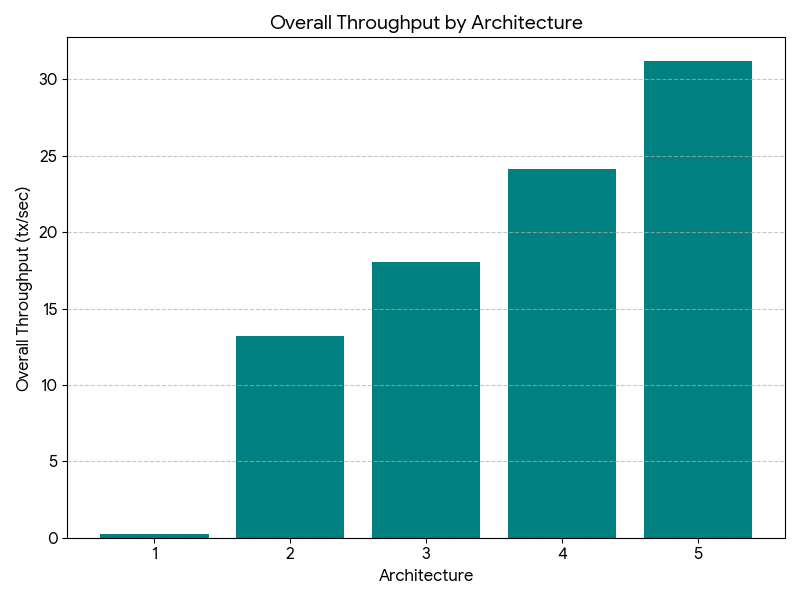
\includegraphics[width=\textwidth]{images/stat1.png}
        \caption{Throughput}
        \label{fig:throughput}
    \end{subfigure}
    \hfill
    \begin{subfigure}[b]{0.32\textwidth}
        \centering
        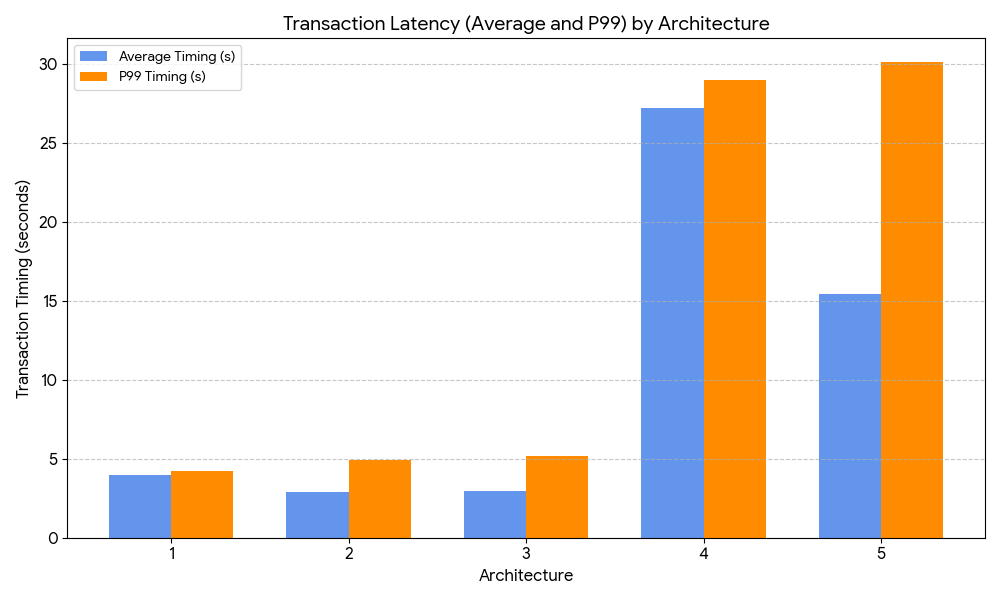
\includegraphics[width=\textwidth]{images/stat2.png}
        \caption{Latency}
        \label{fig:latency}
    \end{subfigure}
    \hfill
    \begin{subfigure}[b]{0.32\textwidth}
        \centering
        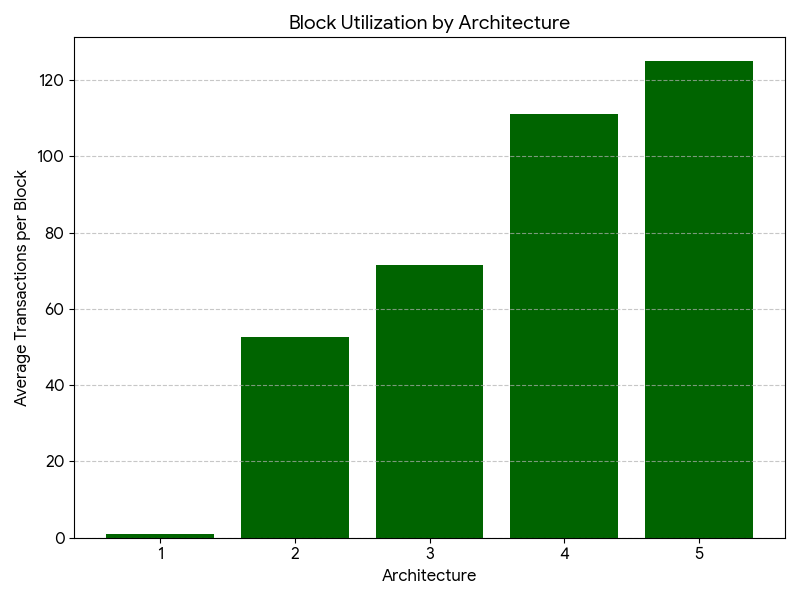
\includegraphics[width=\textwidth]{images/stat3.png}
        \caption{Block Utilization}
        \label{fig:block_utilization}
    \end{subfigure}
    \caption{Performance metrics across architectural stages.}
    \label{fig:performance_metrics}
\end{figure}

\subsection{From Synchronous to Asynchronous: Overcoming Network Latency}

Throughput improved most significantly in the transition from Architecture~1 to Architecture~2. Decoupling submission from synchronous confirmation increased throughput over 50$\times$, from 0.25~tx/sec to 13.22~tx/sec, confirming that the naive implementation was bottlenecked by block time. Average latency dropped from 4.0s to 2.9s as asynchronous submission enabled more efficient transaction batching~\cite{ding2018batching,hennessy2017computer}.

\subsection{The Nonce Bottleneck: The Limits of Single-Wallet Parallelism}

Architecture~3's multi-threaded submission provided a key insight: despite parallel processing, throughput increased only 36\%, from 13.22~tx/sec to 18.04~tx/sec. Because nonce requirements are strictly sequential, threads serialized at the blockchain level, limiting parallelization gains consistent with Amdahl's Law~\cite{amdahl1967validity}. True parallelization requires addressing the single-wallet nonce constraint.

\subsection{Server-Side Contention Emerges}

Architecture~4 introduced a wallet pool to circumvent nonce constraints, increasing throughput to 24.16~tx/sec. However, this came at significant cost: average latency rose sharply from ~3s to over 27s (P99: ~29s). Removing the blockchain-level bottleneck shifted contention to the server~\cite{moir2018concurrent}. Without coordination, threads competed for shared resources, causing cache thrashing and lock convoying; transactions queued locally before reaching the network.

P99 latency (28.97~s) relative to the average (27.21~s) indicates most transactions experienced similar delays, a systemic bottleneck rather than occasional outliers. This pattern is characteristic of lock contention, where threads wait for exclusive access to shared resources.

\subsection{The Proposed Solution: Symbol-Sharding and Lock-Free Queues}

Architecture~5 introduced symbol-sharding and lock-free queues to address server-side contention. This achieved the highest throughput at 31.19~tx/sec (29\% over Architecture~4) while reducing average latency by 43\%, from 27.2s to 15.4s. Partitioning by trading symbol and using CAS-based lock-free queues effectively eliminates server-side resource competition~\cite{harris2001pragmatic}.

P99 latency remained high (~30s), indicating tail latency persists for highly contended symbols that create temporary within-shard backlogs, a challenge for future work.

\subsection{Block Utilization, Burst Handling, and Scalability}

Block utilization rose with throughput improvements: from 1.0~tx/block (baseline) to 125.0~tx/block (Architecture~5). Gas usage remained stable (146,194--152,603 gas/tx), confirming gains were purely architectural.

The observed 125~tx/block exceeds the theoretical maximum of ~71.7~tx/block, demonstrating successful burst handling: the architecture submitted transactions at 1.74$\times$ the blockchain's sustained capacity (~17.93~tx/sec), with excess transactions queuing in the mempool. This is critical for trading workloads where market events trigger sudden order spikes.

The architecture scales linearly with blockchain capacity increases (Layer~2, higher gas limits, faster consensus). Because the submission layer sustains rates exceeding blockchain capacity, symbol-sharded pipelines operate independently with negligible overhead. The submission layer is demonstrably not the bottleneck.

\subsection{Answering the Research Questions}

Our empirical results provide clear answers to each of the research questions posed in the introduction.

\textbf{Answer to RQ1 (Throughput Ceiling and Shifting Bottlenecks):} The throughput ceiling is \textbf{31.19~tx/sec}, a \textbf{2.8$\times$ improvement} over conventional asynchronous multi-threaded designs. The ablation reveals bottlenecks \textit{shifting}: synchronous I/O (Arch~1$\rightarrow$2) $\rightarrow$ nonce serialization (Arch~2$\rightarrow$3) $\rightarrow$ server-side contention (Arch~3$\rightarrow$4) $\rightarrow$ submission layer no longer limiting (Arch~5). This demonstrates \textbf{contributions C3 and C4}.

\textbf{Answer to RQ2 (Adapting HFT Patterns to Blockchain):} Lock-free HFT patterns adapt successfully to blockchain submission with careful nonce co-design. Symbol-sharded, CAS-based queues eliminate server-side contention, though persistent high P99 latency (~30s) indicates within-shard contention for popular symbols remains a challenge (\textbf{contribution C1}).

\textbf{Answer to RQ3 (Architectural Design vs. Latency):} Architectural design significantly impacts settlement latency. The 9$\times$ latency increase from Architecture~3 (2.96s) to Architecture~4 (27.21s) resulted solely from server-side contention (\textbf{contribution C5}). The symbol-sharded design reduced latency by 44\% while increasing throughput, demonstrating that both metrics can improve concurrently.

% References for this section are in the main bibliography


% ============================================
% VIII. THREATS TO VALIDITY
% ============================================
\section{Threats to Validity}

\label{sec:threats}

We follow the framework of Shadish et al.~\cite{shadish2002experimental} to categorize validity threats.

\textbf{Internal Validity:} We strengthened internal validity through our incremental ablation study, isolating each architectural modification's impact. All experiments ran on a dedicated testbed, and consistent gas usage across architectures confirms that performance differences stem from architectural changes rather than on-chain computational variance.

\textbf{Construct Validity:} Our metrics—throughput, latency, and block utilization—are standard performance indicators~\cite{hennessy2017computer}. However, our workload of fixed atomic trades evenly distributed across symbols is a simplification; bursty real-world patterns may yield different results.

\textbf{External Validity:} Our experiments used a private Ethereum network (IBFT 2.0, 4-second blocks), not the public mainnet. This is intentional: we target private/permissioned blockchains used in enterprise settings~\cite{lewis2017blockchain,androulaki2018fabric}. While the principles of nonce bottlenecks, server-side contention, and sharding benefits should generalize, precise quantitative improvements are testbed-specific. The 2.8$\times$ improvement over conventional architectures and the ability to sustain rates exceeding the blockchain's theoretical capacity are the more generalizable findings~\cite{choffnes2010pitfalls}.

\textbf{Research Question Impact.} RQ1's absolute throughput (31.19~tx/sec) is platform-specific, though the migrating bottleneck pattern should persist. RQ2's HFT adaptations (lock-free structures, symbol-sharding) are platform-agnostic. RQ3's 9$\times$ latency increase from contention represents a fundamental systems phenomenon that should manifest across platforms.


% ============================================
% IX. CONCLUSION AND FUTURE WORK
% ============================================
\section{Conclusion and Future Work}
\label{sec:conclusion}

In this paper, we presented a systematic ablation study of architectural patterns for blockchain-based trading, grounded in the production Horizon Globex platform. Our symbol-sharded, lock-free architecture achieves 31.19~tx/sec (\textbf{2.8$\times$ improvement} over conventional designs), with migrating bottlenecks revealing that naive multi-threading yields only 36\% gains due to nonce serialization, and that resolving this with multi-wallet strategies causes a 9$\times$ latency increase from server-side contention.

The symbol-sharded, lock-free model resolves this crisis: 29\% higher throughput with 44\% lower latency, shifting the bottleneck away from the submission layer. Because the submission layer sustains rates exceeding the blockchain's theoretical capacity, the architecture scales linearly with network upgrades.

\subsection{Future Work}

\textbf{Sustained Load Testing.} Our 1,000-transaction workload demonstrated relative architectural performance but did not reach steady-state saturation. Extended tests at rates exceeding the theoretical ceiling (~17.93~tx/sec) would characterize sustained throughput, mempool dynamics, and latency under prolonged load.

\textbf{Maximal Extractable Value (MEV) Mitigation and Fair Ordering.} Our model does not guarantee fair transaction ordering within blocks, leaving it potentially vulnerable to MEV extraction even in permissioned settings~\cite{qin2022mev,ji2024mev}. Future work should explore fair ordering protocols (commit-reveal schemes, threshold encryption) and analyze the fairness-throughput trade-off.

\textbf{Cross-Shard Atomic Trading.} Symbol-sharding does not natively support atomic multi-symbol trades. Cross-shard protocols (2PC or optimistic mechanisms) could enable atomic settlement across shards~\cite{zhang2023frontrunning,du2024crossshard}.

\textbf{Generalizability to Other DLT Platforms.} Benchmarking on other permissioned DLTs, particularly Hyperledger Fabric with its different consensus model, would validate the generalizability of our architectural principles~\cite{ucbas2023performance,baliga2018hyperledger}.


% ============================================
% X. ACKNOWLEDGEMENTS
% ============================================
\section*{Acknowledgements}
This research was funded by Research Ireland under grant number 13/RC/2094 in conjunction with Horizon Globex Ireland DAC. under statement of work SOW2017-055.

\section*{Data Availability}
The source code for all five architectural variants, the smart contract, and the experimental harness are publicly available at: \url{https://github.com/HorizonFintex/blockchain-trading-architectures}.

\section*{AI Usage Statement}
Microsoft Copilot was used to assist with spelling, grammar, and phraseology during manuscript preparation and review. All intellectual content, analysis, and conclusions are the authors' own work. The authors bear full responsibility for the accuracy and integrity of this paper.


% ============================================
% XI. REFERENCES
% ============================================
\bibliographystyle{IEEEtranBST2/IEEEtran}
\bibliography{IEEEtranBST2/IEEEabrv,paper_references}

\end{document}
